\begin{figure}[t]\centering
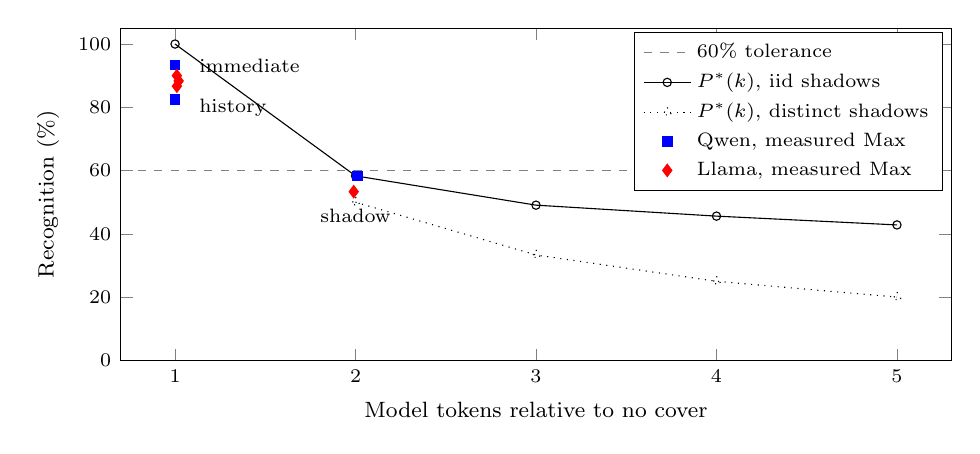
\begin{tikzpicture}
\begin{axis}[width=\columnwidth,height=5.8cm,xmin=0.7,xmax=5.3,ymin=0,ymax=105,
 xlabel={Model tokens relative to no cover},ylabel={Recognition (\%)},
 xtick={1,2,3,4,5},ytick={0,20,40,60,80,100},
 legend style={font=\scriptsize,at={(0.99,0.99)},anchor=north east,cells={anchor=west}},
 tick label style={font=\scriptsize},label style={font=\footnotesize}]
\addplot[gray,dashed,mark=none,domain=0.7:5.3] {60};
\addlegendentry{60\% tolerance}
\addplot[black,mark=o,mark size=1.5pt] coordinates {(1,100) (2,58.33) (3,49.07) (4,45.60) (5,42.82)};
\addlegendentry{$P^*(k)$, iid shadows}
\addplot[black,dotted,mark=triangle,mark size=1.8pt] coordinates {(2,50) (3,33.33) (4,25) (5,20)};
\addlegendentry{$P^*(k)$, distinct shadows}
\addplot[only marks,blue,mark=square*,mark size=1.7pt] coordinates {(1,93.33) (1,82.5) (1,82.5) (2.01,58.33)};
\addlegendentry{Qwen, measured Max}
\addplot[only marks,red,mark=diamond*,mark size=2.2pt] coordinates {(1.01,90) (1.01,86.67) (1.02,88.33) (1.99,53.33)};
\addlegendentry{Llama, measured Max}
\node[font=\scriptsize,anchor=west] at (axis cs:1.08,93) {immediate};
\node[font=\scriptsize,anchor=west] at (axis cs:1.08,80) {history};
\node[font=\scriptsize,anchor=north] at (axis cs:2,51) {shadow};
\end{axis}
\end{tikzpicture}
\caption{Inference versus model work against the call-window observer. Points are the strongest tested attacks for the four cover arms; lines are derived plausible-deniability floors for $k=0$--4 shadows, not measurements. Only $k=1$ with iid labels was measured. Controller cover costs no model work but leaves 83--93\% recognition; the measured shadow sits on its floor.}\label{fig:frontier}
\end{figure}
